\chapter{Receiver-Driven View-Dependent Streaming of Progressive Meshes}
\label{c:rdstream}
\section{Introduction}
\label{s:dstream:intro}
    During streaming of a progressive mesh, it is desirable to 
    increase the visual quality of the reconstructed mesh in the client side
    as quickly as possible. 
    Therefore, vertex splits having high contribution to the visual quality
    should be sent early. 
    What the user really can see, however, is not the mesh itself but the rendered
    image on the screen. The quality of the rendered image
    depends on not only the quality of the mesh but also the viewpoint
    of the user. The contribution of a vertex split, as a result, 
    also depends on the viewpoint of the user. 
    Hence, using quality metrics independent of viewpoint,
    such as the commonly used Hausdorff distance between the 
    original and reconstructed mesh \cite{cignoni98metro}, to
    decide the streaming order, is not accurate enough. 
    %One solution is to send the vertex splits
    %in the descending order of their contribution to
    %mesh quality, commonly measured by the Hausdorff distance between
    %the original and reconstructed mesh \cite{cignoni98metro}.
    %As Hausdorff distance is view independent, 
    Bandwidth may be wasted in sending invisible vertex splits
    before the visible ones. Moreover, even among the visible vertex splits,
    the view-independent metric cannot reflect the real contribution to
    the visual quality of rendered images in clients with different viewpoints. 
    A vertex split that significantly changes a mesh may change the rendered image 
    only slightly.

    A better metric of the visual contribution of a vertex split, 
    which considers the receiver's viewpoint, is 
    based on the quality of the rendered image on the screen.
    An example is the one proposed by Lindstrom and Turk \cite{353995}.
    Based on this view dependent metric, \emph{view-dependent} streaming,
    in which vertex splits are sent in the descending order of 
    their contributions to the quality of rendered image, is introduced
    to improve the user experience. 
    
    \begin{figure}
    \centering
    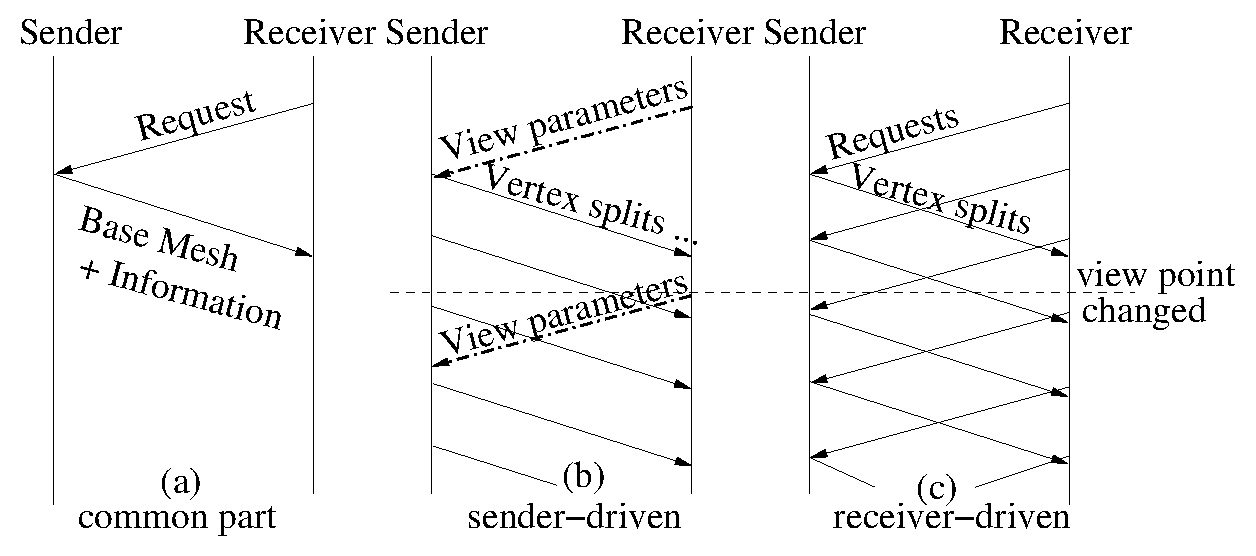
\epsfig{file = protocol.eps, width = 0.75\textwidth}
    \caption{Sender-driven protocol and receiver-driven protocol 
    \label{dstream:protocol}}
    \end{figure}
    In previous implementations of view dependent streaming
    \cite{To1999, 363375, progressive:Yang, kim:view, zheng:interactive}, 
    the sender decides which vertex splits to send. In these implementations,  
    the receiver sends its viewing parameters to the sender, 
    and the sender sends the chosen vertex splits after
    determining the visibility and the appropriate resolution of 
    different regions of the mesh (See Figure \ref{dstream:protocol}b).

    This sender-driven protocol is not scalable to a large number 
    of receivers (unless using more servers as senders, 
    which significantly increases the infrastructural cost) 
    due to its two characteristics:
    (1), the sender is state-ful because it needs to remember which
    vertices are sent for each receiver to avoid sending duplicate data
    when receivers changes viewpoint;
    (2), the sender has to do expensive computation to determine the 
    visibility and visual contributions of vertex splits for each receiver.
    
    Due to the state-ful design and huge computational requirements,
    the sender-driven approach cannot be extended easily to support 
    caching proxy and peer-to-peer architecture, two common solutions to scalability. 
    First, it is difficult for a receiver to request data from multiple proxies or peers
    without receiving duplicate data.
    Second, it is not realistic to require each proxy or peer to provide much CPU (or even GPU) time
    and memory (maintaining state of other receivers) to other receivers. 
    Third, a proxy or peer might not store the complete mesh for visibility determination.

    To address the above weaknesses and design a more scalable view dependent streaming system, 
    we propose a receiver-driven protocol, 
    in which the receiver decides the sending order and explicitly requests
    the vertex splits. The sender simply sends the data requested 
    (See Figure\ref{dstream:protocol}c), so no expensive computation is needed.
    %In this protocol, the server is stateless and free of expensive computation.
    %We can exploit the client's GPU in determining the requesting order.
    Furthermore, the server is stateless, so
    existing cache proxy and peer-to-peer techniques can be applied.

    \begin{comment}
    The receiver-driven protocol also reduces the size of data sent by the sender.
    In sender-driven protocols, for each vertex split, the sender has to send identifications
    to indicate which vertex to be split ($V_s$ in Figure \ref{f:intro:split2}),
    requiring at least $log_2{n}$ bits if $n$ vertices exist \cite{258843}. 
    In the receiver-driven protocol, however, the sender needs not send
    these identifications since the vertex splits can be sent according to
    the requesting order from the receiver. The identifications, sent
    by the receiver, consumes the down-link bandwidth 
    of the sender, which is often less likely to be the bottleneck than the up-link.
    \end{comment}

    Implementing the receiver-driven protocol is non-trivial. It introduces some 
    new research questions.
    First, the receiver has to efficiently determine the visibility and visual contribution
    of a vertex split based on partially received mesh. 
    Second, we need to assign each vertex a unique identification number
    so that the receiver can explicitly request vertex splits. 
    To avoid sending extra data, the identification number of each vertex 
    should implicitly known by the receiver.
    %Although it is difficult for the receiver to accurately measure
    %the visual importance of a vertex split, we find that estimation suffices
    %in our scheme.  
    Third, most current coding and compression methods exploit the sending order of vertex splits
    to increase the compression efficiency as we introduced in Chapter \ref{c:related}.
    We now, however, need a new compression scheme
    completely independent of the sending order since the sender has no freedom in choosing sending order.

    To explain why receiver-driven approach introduce the new research questions,
    we briefly introduce how these questions are solved in current sender-driven approaches and 
    why these methods are not applicable in receiver-driven approach in Section \ref{s:dstream:terms}.
    %Before we introduce our solutions, we briefly review the current view-dependent approaches,
    %so we can see why receiver-driven protocol introduce new research problems and challenges. 
    Then, we present our solutions of these problems in Section \ref{s:dstream:protocol}.
    We validate our solutions by experiments in Section \ref{s:dstream:evaluation} 
    and conclude in Section \ref{s:dstream:conclude}.

%\section{Current View-dependent Approaches}
\section{Problem Statement}
\label{s:dstream:terms}
    \subsection{Determine Visibility and/or Visual Contribution of a vertex split}
    We first define a term \emph{the visibility of a vertex split}. Under a certain
    viewpoint, if split a vertex will help improving the quality of the rendered image,
    we call this vertex split \emph{visible}. Otherwise, we call it a \emph{invisible}
    vertex splits.
    In view-dependent streaming system, it is necessary to determine the visibility
    of each vertex split so that the sender can avoid wasting bandwidth in sending invisible 
    vertex splits and use the saved bandwidth to send more visible vertex splits.

    The visibility of a vertex split is not simply the visibility of the \emph{corresponding
    vertex} (the vertex to be split by the vertex split), because splitting an invisible
    vertex may generate visible vertices and improve the quality of the rendered image. 
    To further illustrate this point, we introduce the term \emph{vertex hierarchy}.
    %In this section, we briefly review the current view-dependent approaches since 
    %they are the basis of our scheme. When we introduce some methods used in the current approaches, 
    %we will point out whether or not (and why) they can be applied to receiver-driven
    %protocol.
    %We first introduce 
    \begin{figure}
    \centering
    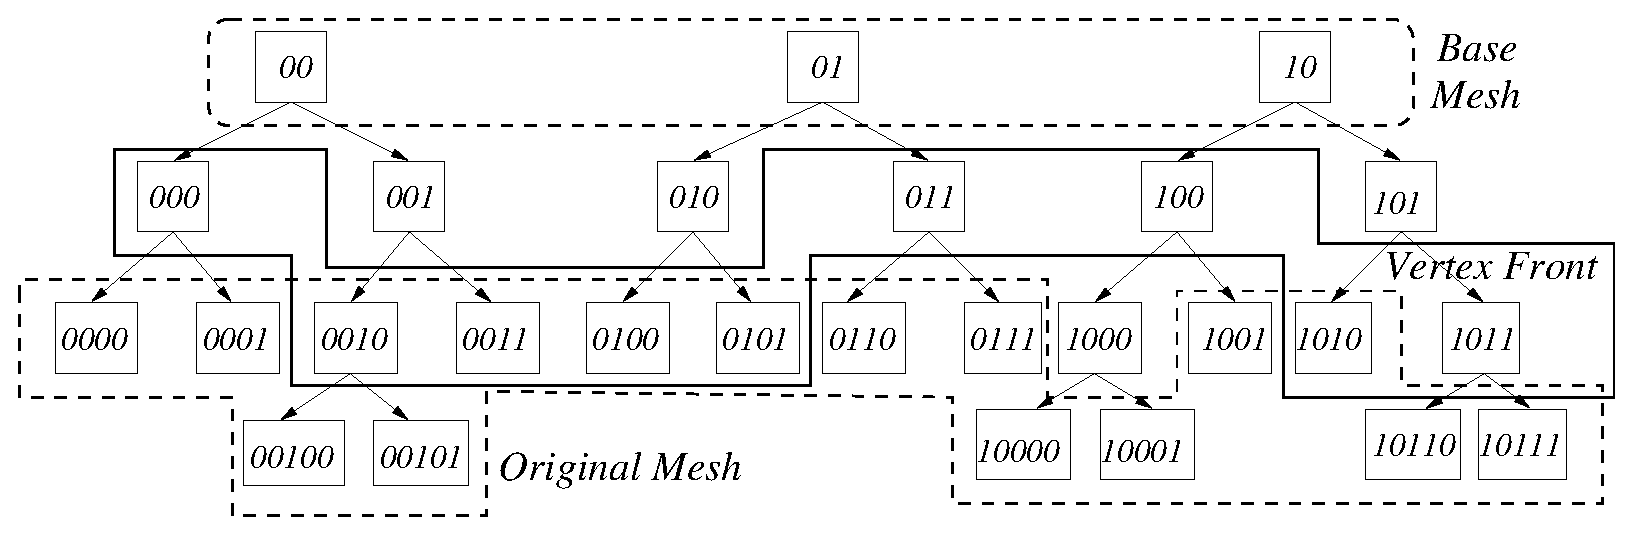
\epsfig{file = hierarchy.eps, width = 0.9\textwidth}
    \caption{Vertex hierarchy and vertex front. A rectangle represents a vertex and the number inside
    is its identification number, including tree ID and node ID.\label{dstream:hierarchy}}
    \end{figure}
    %View-dependent systems often organize the vertices hierarchically.
    Vertex splits in a progressive mesh can be organized hierarchically.
    For example, Hoppe \cite{258843} represents
    parent-child relation among the vertices in a progressive mesh
    as a forest of binary trees, named \emph{vertex hierarchy},
    in which the root nodes are vertices in the base mesh, and
    the leaf nodes are vertices in the original mesh (see Figure \ref{dstream:hierarchy}).
    A vertex split replaces one vertex ($V_s$ in Figure \ref{dstream:split})
    by its two children ($V_u$ and $V_t$ in Figure \ref{dstream:split}).
    Thus, after applying some vertex splits,
    the result is a mesh lying between the original mesh and the base mesh.
    The set of vertices in current mesh is called \emph{vertex front}
    \cite{258843}
    (see Figure \ref{dstream:hierarchy}).% and vertices in the vertex front are \emph{active vertices}
    
    %When determining the visibility of vertex splits, a vertex split cannot be ignored when it
    %is not visible. If any of its descendants in the vertex hierarchy is visible,
    %the vertex split still needs to be applied. To avoid determining the visibility
    %Due to dependencies among the vertices, visibility determination of a vertex cannot be based 
	%on this vertex alone.
    Therefore, an invisible vertex still needs to be split if any of its descendants is visible. 
    To avoid determining the visibility %\footnote{
    %For simplicity, in this paper determining the visibility also includes computing screen-space error.} for each
    recursively for all the descendants,
    %vertex in the vertex hierarchy is expensive. Therefore, 
    a common method is to use a bounding sphere to include a vertex and all its descendants.
    Then, we can safely ignore a vertex split if its bounding sphere
    falls outside the view frustum.
    Similarly, a bounding cone of normal is used in back face culling \cite{258843}.
    Therefore, some extra information to represent the bounding sphere
    and bounding cone of normal is needed. Both Hoppe and Kim et al. \cite{258843, kim:view}
    pre-compute the radius of the bounding sphere ($r_v$), the semi-angle of
    the cone of normals ($\alpha$), and other two parameters
    ($\mu$ and $\delta$) for deciding the screen-space error
    and store them with the vertex together.
    
    These bounding object-based methods, however, are not appropriate
    in our receiver-driven protocol. 
    If these methods are applied to receiver driven protocol, the sender has to send
    these bounding parameters with the vertex splits, almost doubling 
    the data size. 
    %To increase the streaming data size is never a good solution
    %because the network bandwidth is one of the main bottleneck of the streaming system.
    We need a method for the receiver to estimate the visibility and contribution of 
    splitting a vertex without extra information.
    We explain our solution to this issue in Section \ref{s:dstream:protocol}.
    %and the transmitted data size will be significantly increased. 
    %Since one vertex split has only five parameters, 
    %the identifications of two cut neighbors ($V_l$ and $V_r$) and the coordinations
    %of the new vertex ($x$, $y$, and $z$)
    %\footnote{We apply the half-edge collapse in our implementation
    %so that only coordinates of one vertex needs to be transmitted.},
    %adding four parameters almost doubles the data size. 
    %It is not acceptable since the network bandwidth
    %is considered as the main bottleneck.  

    \subsection{Identify Vertices}
    After deciding the visibility, the sender sends the chosen vertex splits to the receiver.
    Six parameters are needed in a vertex split of a manifold mesh: the identification number
    (we call ID from now on) of the vertex to be split
    ($V_s$ in Figure \ref{dstream:split}) $Ids$, 
    the IDs for two cut neighbors 
    ($V_l$ and $V_r$ in Figure \ref{dstream:split}), $Id_l$ and $Id_r$,
    and the coordinates $x$, $y$, and $z$ of the right child ($V_t$ in
    Figure \ref{dstream:split}). Here, half collapse is used so $V_u$ remains at the same position
    of $V_s$. 
    
    Many sender-driven implementations use the sequence number of a vertex generated as its ID,
    then the IDs of two newly generated vertices can be implicitly known by the receiver without
    extra information. This method, however, 
    enforces the sender to be state-ful since the sender has to remember 
    the sending order of vertex splits for each receiver. 
    Therefore, it is not applicable in our receiver-driven protocol.
    \begin{figure}
    \centering
    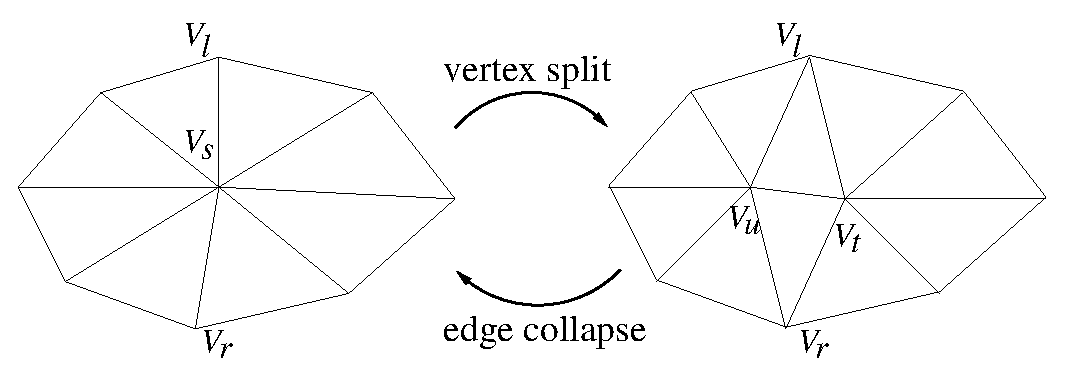
\epsfig{file=split.eps, width=0.6\textwidth}
    \caption{A vertex split split $V_s$ to $V_t$ and $V_u$, with $V_l$ and $V_r$ as two cut neighbors.}
    \label{dstream:split}
    \end{figure}

    Kim and Lee \cite{kim01truly} proposed a new method, in which every vertex has
    an ID that is independent of the sending order. The ID of a vertex is a bit string
    with two parts: tree ID and node ID.
    Tree ID is the sequence number of the root of this tree in the base mesh, 
    and the node ID represents the path from the root to this vertex in the binary tree.
    For example, if the tree ID is `01', which is also the ID of
    the root vertex of this tree, the bit string `010' and `011' are the IDs
    of the left child and right child of the root vertex respectively. 
    A vertex hierarchy with the assigned IDs is shown in 
    Figure \ref{dstream:hierarchy}.

    Besides being independent of the sending order, another benefit of this scheme
    is that the IDs embed the hierarchy. Thus,  
    we can deduce the IDs of the ancestors and the descendants of each vertex. 
    For example, given `1001' as the ID of a vertex,
    we can deduce that `100' is the ID of its parent, `10010' is the ID of its left child and 
    `10011' is the ID of its right child. 
    This property frees the sender from sending the IDs of the two newly generated vertices
    ($V_u$ and $V_t$ in Figure \ref{dstream:split}), as they can be deduced by the receiver.

    As a result, with Kim and Lee's method \cite{kim01truly}, we can identify the vertices
    implicitly and the identification numbers are independent of the sending order of the 
    vertex splits, which is essential to ensure the sender is stateless.

    \subsection{Compress Vertex Splits Efficiently}
    As we introduced above, in a sender-driven protocol, 
    a vertex split usually includes five numbers {$IDs$, $ID_l$, $ID_r$,
    $x$, $y$, $z$}. 
    In the receiver-driven protocol, on one hand, the sender needs not send
    $IDs$ since the vertex splits can be sent according to
    the requesting order from the receiver. On the other hand, the other 
    five numbers are more difficult to be compressed efficiently.
    
    \textbf{Encoding $ID_l$ and $ID_r$}

    In sender-driven protocol, instead of sending the two cut neighbors, $ID_l$ and $ID_r$, directly,
    only the information indicating their position among all the \emph{one ring neighbors}
    of vertex $IDs$ (the vertices directly connected to vertex $IDs$) is coded.  
    Since the number of one ring neighbors is much smaller than the total number of vertices,
    much less bits are needed than coding $ID_l$ and $ID_r$ directly. Moreover, entropy coding
    can be used to further improve coding efficiency because the vertex $ID_l$ and vertex $ID_r$
    are not equally possible in any position.

    In the receiver-driven approach, however, the method introduced above is not applicable.
    Because the receiver may split the progressive mesh in many ways, the set of neighbors of 
    a vertex during the decoding, $\mathcal{N}'$, 
    may not be the set of neighbors during the encoding $\mathcal{N}$.
    Moreover, a stateless sender does not remember the sending
    order, so it has no idea what the set is. 
    As a result, even coding on the fly is not possible. 
    In the receiver-driven approach, $ID_l$ and $ID_r$ need to be encoded independent to the decoding order. 

    
    Kim et al. \cite{multiresolution:kim} proposed an efficient algorithm to encode the IDs
    of two cut neighbors. With their method, the proper cut neighbors can be selected from
    the one ring neighbors $\mathcal{N}'$, no matter what $\mathcal{N}'$ is that time. 
    Moreover, even the vertex $ID_l$ or vertex $ID_r$ itself is not in $\mathcal{N'}$ that
    time, the vertex split still could be applied properly.
    Their method is based on the following observation.
    %The above property is also essential in splitting
    %Ta progressive mesh in random order, in which the set of neighbors of a vertex
    %during the decoding $\mathcal{N}'$ may not be $\mathcal{N}$, the set 
    %during the encoding. 
    If a cut neighbor vertex with an ID of $Id$ %in $\mathcal{N}$
    is not in $\mathcal{N}'$, then either one of its 
    ancestors or at least one of its descendants must belong to $\mathcal{N}'$ \cite{multiresolution:kim}.
    In the former case, the ancestor is found and used as 
    the cut neighbor since its ID is the prefix of $Id$.  
    In the latter case, the descendants of the original 
    cut neighbor in $\mathcal{N}'$ are found since they all have $Id$ as their prefix.
    Kim et al. \cite{multiresolution:kim} propose a method to find out the 
    proper one as the cut neighbor and they show that despite using replacement
    in the vertex splitting, the original mesh can be 
    accurately reconstructed when all the vertex splits are applied.

    Kim et al. \cite{multiresolution:kim} also propose an algorithm
    to encode the IDs of two cut neighbors at about 12 bpv (bit per vertex) 
    %and the coordinates $x$, $y$, and $z$ at about 21 bpv 
    (with 12 bit quantization).
    Although their paper focuses on random access of local meshes, we find that this 
	method is useful in progressive streaming as well. 
    
    \textbf{Encoding ($x$, $y$, $z$)}
    As we introduced in Chapter \ref{c:related}, the coordinates of the newly generated
    vertex, ($x$, $y$, $z$) can be encoded based on the prediction. Usually, the prediction
    is based on position of some other vertices close to the vertex $IDs$. This method is 
    not applicable in the receiver-driven approach. Now, because of the random splitting order, 
    it is possible that those vertices do not exist yet when vertex $IDs$ is split. 
    
    We proposed a simple method to encode the $x$, $y$, $z$ based on the position
    of its parent, the vertex $IDs$ itself. First, the child is usually close to its
    parent. Second, the parent, vertex $IDs$ here, definitely exist. Otherwise, the vertex
    split cannot be applied anyway. 

    We will introduce our implementation of encoding ($ID_l$, $ID_r$, $x$, $y$, $z$) 
    in detail in Section \ref{s:dstream:protocol}.

\section{Receiver-Driven Protocol}
     \label{s:dstream:protocol}
	 We now present our proposed receiver-driven protocol
     for view-dependent progressive mesh streaming.
     We first introduce the process of transmitting 
     a progressive mesh. Then, we explain how the receiver decides the requesting order.
     Finally, we explain how we efficiently encode the request from the receiver.
     
     \subsection{Mesh Transmission} 
     A streaming session is initiated when the receiver requests for a specific
     mesh.
     The sender returns the complete base mesh and other necessary information,
     such as the Huffman tables used in decoding vertex splits, to the receiver
     (See Figure \ref{dstream:protocol}a).
     
     \begin{figure}
     \centering
     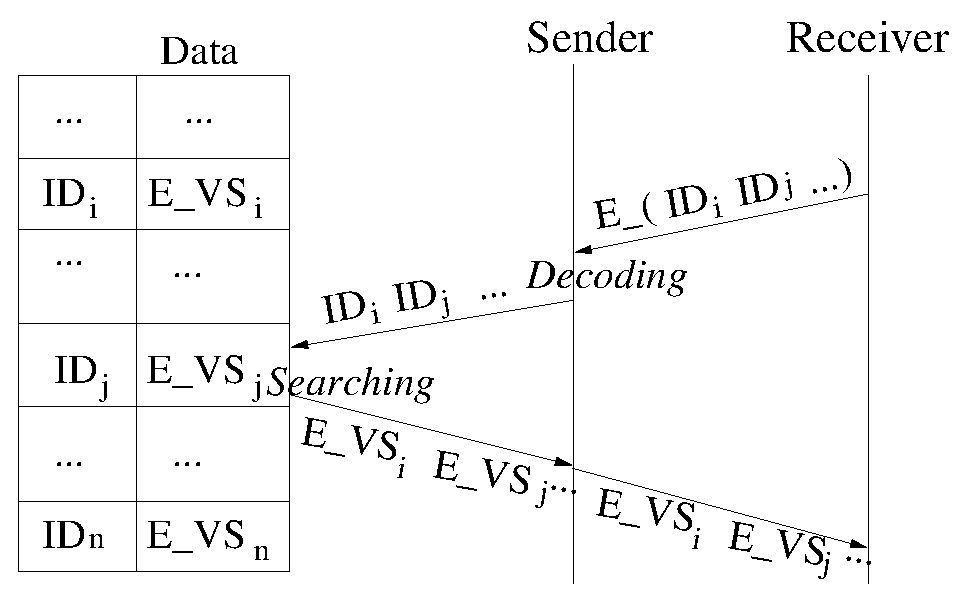
\epsfig{file =process.eps, width=0.5\textwidth}
     \caption{The process of the sender in receiver-driven protocol. 
     E represents encoded data, and VS means vertex split. \label{dstream:process}}
     \end{figure}
     %After receiving the base mesh, 
     Then, the receiver determines
     the requesting order of the vertex splits based on the received base mesh, 
     encodes their IDs, and
     sends them to the sender. On the sender side, the vertex splits are stored
     in an associative array, which maps the ID to the vertex splits. 
     After receiving the encoded IDs from the receiver, 
     the sender decodes the IDs and searches for the vertex splits 
     in the associative array
     with IDs as the key values. The matched vertex splits
     are sent back to the receiver (See Figure \ref{dstream:process}). 
     The sender does only two things -- decode IDs and retrieve the 
     vertex splits, and is therefore stateless. 

     To avoid the receiver to request a non-exist vertex split (that is to split
     a leaf vertex in the vertex hierarchy),
     an extra bit is attached to every vertex to indicate whether it is leaf or not.
     This will be introduced in more detail when we discussing about coding vertex splits
     later.
     
     \subsection{Determining Visual Importance}
     \label{ss:dstream:visual}
     We now introduce how the receiver decides the requesting order. 
     %We cannot directly use the mean square error between rendered images of 
     %reconstructed mesh and original mesh to determine the order, 
     %image-based metric proposed by Lindstrom and 
     %Turk \cite{353995} 
     We cannot know exactly the contribution of a vertex split in the receiver side
     because it is not received yet when it is requested.
     Adding extra information, such as the radius of bounding sphere, is not appropriate
     because it will significantly increase the data size. 
     Therefore, we can only estimate the contribution of vertex splits based on the 
     partially received mesh.
     
    \begin{figure}
    \centering
    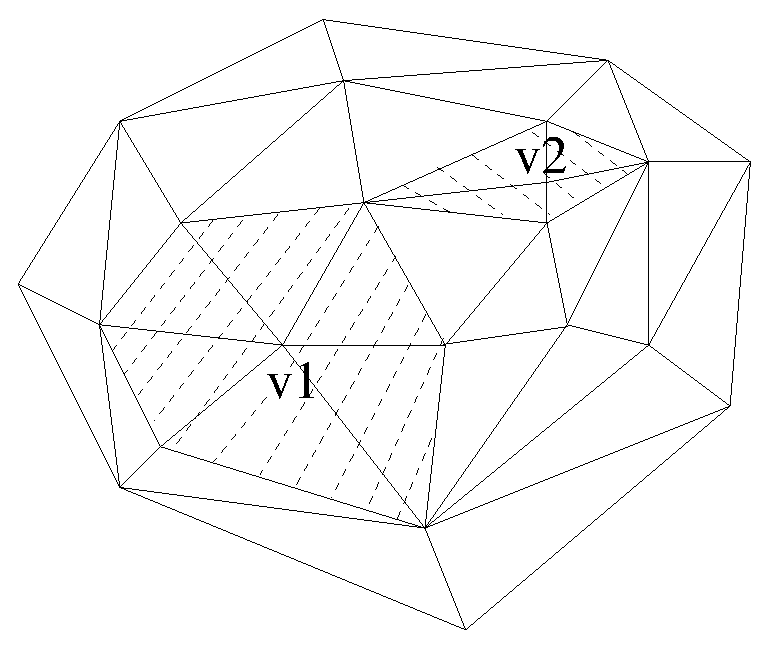
\epsfig{file =screen_area.eps, width=0.35\textwidth}
    \caption{Rendered image on the receiver's screen. 
    The shaded are the screen area of vertex $V_1$ and vertex $V_2$.
    \label{dstream:screen_area}}
    \end{figure}
     We propose to use the screen-space area of all the neighbor faces of a vertex as the 
     metric of its visual importance (see Figure \ref{dstream:screen_area}).
     The rationale is that if the screen area of a vertex ($V_1$ in Figure \ref{dstream:screen_area}) 
    is larger, it is likely the quality can be improved more by splitting this vertex. 
    
    We compute the screen-space area with the help of the GPU. 
    First we assign each face in the current mesh a unique color and render them. 
    We can determine the visibility
    and the screen-space area of each vertex by counting how many pixels with its color
    are in the frame buffer, where the rendering result is stored. 
    Then we add the pixel number to the face's three vertices. Thus, the
    pixel number of a vertex (which is the sum of pixel numbers in its neighbor faces)
    is proportional to its screen-space area.
    This process introduce some delay, but the delay can be compensated by the time
    we saved from rendering only visible part of a large mesh later. 
    
    After the screen-space areas are computed, 
    the receiver sends the requests following the descending order of the 
    screen-space area. If the viewpoint changes, the visual importance will
    be re-computed and a new list of vertex splits will be requested. Since the received
    splits refine the mesh, the receiver recomputes the visual importance periodically
    to update the order even without viewpoint change. The refresh period, one second
    in our experiments, can be decided
    by the receiver based on mesh size and network bandwidth.

    Once the receiver satisfies with the rendering quality, it 
    can either stop requesting or continue requesting the remaining vertex splits
    for future use based on the prediction of the user's next action. 
    In Chapter \ref{c:user}, we discuss about whether the user actions can be predicted.

    If the receiver stops requesting % for more vertex splits 
    when the visual quality is satisfactory, it may miss some visible vertices.
    As we introduced in Section \ref{s:dstream:terms}, we cannot simply ignore 
    all invisible vertices, because they may have visible descendants.
    Unlike sender-driven approach, where the visibility of a vertex and its all descendants
    can be determined with its bounding sphere, we estimate the visibility of 
    a vertex and its descendants based on the visibility of its neighbor faces. 
    This estimation may introduce some error (mostly on the silhouette), 
    but fortunately, in most cases this kind of error is small and tolerable
    (See the experiment results in Section \ref{s:dstream:evaluation}).
    If strict accuracy is needed, the receiver can choose to continue requesting 
    for the remaining vertex splits.  
		%Furthermore, some methods may reduce 
    %this kind of error, for example, by generating an appropriate base mesh or giving more
    %weight to the silhouette. We will consider these techniques in the future. 
    
    \subsection{Encoding of Vertex Splits and IDs}
    \label{ss:dstream:encoding}

    %Our progressive meshes are generated using OpenMesh\footnote{http://www.openmesh.org}. 
    %Here, we consider only manifold meshes and use half collapse in the simplification. We 
    %%The happy Buddha mesh is from Stanford University.
    %also use Kim's algorithm \cite{multiresolution:kim}
    %to code the IDs of two cut neighbors ($Id_l$ and $Id_r$).
	In this section, we explain how we encode the vertex splits 
    and the IDs of the requested vertex splits.  
    Note that, in our work, we consider only manifold meshes and use half 
	collapse in the simplification.
    
    \textbf{Encoding Vertex Splits}
	To encode a vertex split, we need to encode the IDs of the two
	cut neighbors and its $x$, $y$, and $z$ coordinates.
	%We use Kim's algorithm \cite{multiresolution:kim} to code
	%the IDs of the cut neighbors.
    We use Kim et al.'s algorithm \cite{multiresolution:kim}
    to encode the IDs of the cut neighbors ($Id_l$ and $Id_r$). 
    Since the neighbors of a vertex is a much smaller set 
    than the whole vertices, a shorter code than the ID is sufficient
    to differentiate the cut neighbors from other neighbors. 
    Let $\mathcal{N}$ represents the set of the IDs 
    (Here IDs are bit strings begin with the first bit after leading 1)
    of the neighbors of $V_s$, the vertex to be split. 
    Then we encode the $Id_l$ and $Id_r$ one by one 
    (if one cut neighbor does not exist, we set its ID as $0$)
    with Algorithm \ref{a:encode_neighbor}.
    \begin{algorithm}
    \caption{Encoding the ID of a Cut Neighbor $Id$. 
    Input: $\mathcal{N}$ and $Id$($Id_l$ or $Id_r$); Output: a bit string \emph{code}.
    \label{a:encode_neighbor}}
    \begin{algorithmic}
    \STATE let $i = 1$;
    \WHILE{$\mathcal{N}$ has more than one member}
        \STATE delete the IDs in $N$ with $i$th bit (counting from the left) different from the $i$th bit of $Id$;
        \IF{any ID is deleted}
            \STATE insert the $i$th bit of $Id$ to the \emph{code};
        \ENDIF
        \STATE $i=i+1$;
    \ENDWHILE
    \end{algorithmic}
    \end{algorithm}
    In brief, each bit in the \emph{code} excludes one or more neighbors
    from $\mathcal{N}$ until only the cut neighbor with $Id$ is left. 
    In ideal case, each bit excludes half of the members
    in $\mathcal{N}$, so the code length is $log_{2}d$, 
    where $d$ is the number of neighbors.
    In worst case, each bit of the code only excludes one neighbor,
    so the code length is $d-1$. 
    After obtaining the two codes for $Id_l$ and $Id_r$, we encode them with Huffman coding algorithm.

    The decoding of these two codes is tricky. %not simply the reverse of the encoding.
    Since we enable splitting a mesh in random order, the set of neighbors of a vertex
    during the decoding $\mathcal{N}'$ may not be $\mathcal{N}$, the set during the encoding.
    If a cut neighbor with ID as $Id$ %in $\mathcal{N}$
    is not in $\mathcal{N}'$, then either one of its 
    ancestors or some of its descendants are in $\mathcal{N}'$ \cite{multiresolution:kim}.
    In former case, with the \emph{code}, the ancestor can be found and used as 
    the cut neighbor since its ID is the prefix of $Id$ 
    (recall the property of the unique identification number scheme).
    %Some bits of the code may not used since they are supposed to
    %be used to differentiate the descendants of this neighbor.
    %We will save these unused bits for future use.
    In latter case, with the \emph{code} we find the descendants of the original 
    cut neighbor in $\mathcal{N}'$ since they all have $Id$ as their prefix.
    Kim et al. \cite{multiresolution:kim} propose a method to find out the 
    proper one as the cut neighbor and they show that despite using replacement
    in the vertex splitting, the original mesh can be 
    reconstructed with all the vertex splits are applied. It is also verified 
    by us both in theory and experiments.
    
    To encode the coordinates, instead of encoding $x$, $y$, and $z$ directly, 
    we encode $dx$, $dy$, and $dz$ with Huffman coding algorithm. 
    Here $dx = x - x_0$, $dy = y - y_0$, 
    and $dz = z - z_0$, and $x_0$, $y_0$, and $z_0$ are the coordinates of
    $V_s$, the vertex to be split. 
    The rationale to code the differences is that they have less entropy, especially
    for the later part of vertex splits, which only change the coordinates slightly.
    It is worth noting that all the encoding process are done off-line and the 
    encoded vertex splits are stored in the associative array, so the encoding will
    not increase overhead to the sender.

    According to the results of our experiments with the Stanford Happy Buddha model,
    we can quantize $dx$, $dy$, and $dz$ to 14 bits. 
    We need 11 bpv for both $Id_l$ and $Id_r$ 
    and 20 bpv for all three of $dx$, $dy$, and $dz$ on average.
    It is worth noting that more bits are needed for $dx$, $dy$, and $dz$ 
    for the earlier vertex splits (about 30 to 35 bpv)
    since their values are larger. 
    The number of bits needed decreases significantly for later part of the vertex splits
    as $dx$, $dy$, and $dz$ decrease. We think that compressing $x$, $y$, and $z$ 
    based on better prediction techniques may further increase the 
    efficiency and it will be an interesting topic of future work.

    \textbf{Encoding IDs of vertex splits}
    We now introduce how we encode the vertex split IDs sent from the receiver to the
    sender. Since we use an 32bit integer to represent an ID,  32 bpv is needed for each ID
    without compression.  
    %First we choose the number of vertex identifications to be packetized appropriately
    %such that their vertex splits after encoded will no exceed
    %the size of an Ethernet packet (often 1500 bytes). The reason is to
    %reduce the dependency among packets so that
    %one packet loss will not affect the decoding of another packet.
    %A previous paper \cite{1291399} has discussed the importance to reduce the dependency
    %among the packets.
    The two parts of an ID, tree ID and node ID, are encoded separately.  
    We use a bit string \textit{code} to store the encoded result.
    First, we sort the IDs in a packet according to the tree IDs, in increasing order. 
    Then, we store the first tree ID to \textit{code} and 
    store each of the following tree ID as the difference from the previous tree ID.
    Since they are sorted, the differences are positive and relatively small numbers.

    \begin{figure}
    \centering
    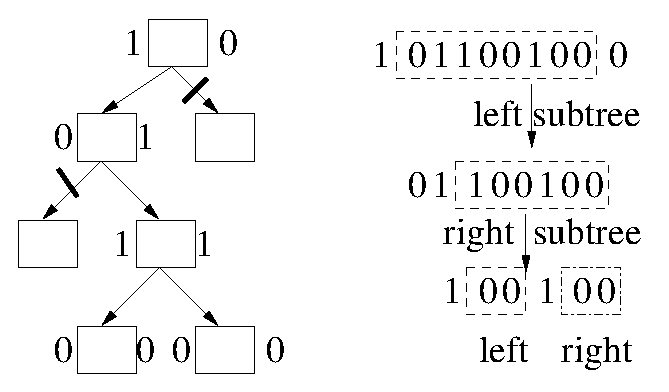
\epsfig{file =encode_id.eps, width=0.4\textwidth}
    \caption{The code of ID of the bottom two
    vertices is 1011001000. 
    \label{f:dstream:encode_id}}
    \end{figure}
    \begin{algorithm}
    \caption{Encoding Vertices in One Tree.
    Input: IDs of vertices in a tree to be split;
    Output: a bit string as the \emph{code}.\label{a:dstream:encode_id}}
    \begin{algorithmic}
    \IF{no vertex needs to be encode in the left subtree}
        \STATE append `0' to \emph{code};
    \ELSE
        \STATE append `1' to \emph{code};
        \STATE encode the left subtree;
    \ENDIF
    \IF{no vertex needs to be encode in the right subtree}
        \STATE append `0' to \emph{code};
    \ELSE
        \STATE append `1' to \emph{code};
        \STATE encode the right subtree;
    \ENDIF
    \end{algorithmic}
    \end{algorithm}
    Next, we encode the node IDs in a tree into a bit string with 
    a recursive algorithm (See Algorithm \ref{a:dstream:encode_id}).
    In brief, we use two bits to represent whether one or more descendants need
    to be split (`1' for yes and `0' for no)
    in the left subtree and right subtree respectively. 
    In the example shown in Figure \ref{f:dstream:encode_id}, for the root vertex, since at least one vertex
    in the left subtree needs to be split, we append `1' to the code and encode the
    left subtree. At the root of the left subtree, since no vertex needs to split in its left
    subtree, we append `0' and check its right subtree. Vertices to be split exist in the right
    subtree, so we append `1' and encode its right subtree recursively as `100100'. 
    Finally, we return back to the root and append `0' since 
    no nodes in the right subtree needs to be split. 
    Therefore, the result is `1011001000'.
        
    During decoding, the sender traverses the tree according to the bits of the code. 
    The bit `1' means to decode the subtree and the bit `0' means to stop and return.
    If a vertex has no descendants that needs to be decoded, then this vertex is split. 
    Decoding is done when the procedure returns to the roots.
    
    The advantage of this method is that the code length is variable and the 
    length can be determined without extra flags. The coding efficiency depends
    on how many vertices need to be split inside a tree. Two bits
    are assigned to each vertex traversed during the encoding
    (including the vertices to be split and their ancestors in their path
    to the roots). Thus, the code efficiency is higher when more vertices in one tree
    are encoded since the overhead is amortized across the vertices. 
    %In worst case, we traverse $d$ nodes just for encoding $1$ vertex,
    %so in maximum $2d$ bits are needed for a node ID. Here, $d$ is
    %the depth of a node. In best case, all leaves are needed to be split. 
    %Assuming there are $m$ leaves, then the
    %total traversed nodes are $2m-1$ and the total bits are $4m-2$.
    %Therefore, in minimum about $4$ bits is needed
    %to encode a node ID. 
    %
    %Due to the limited space, we omit the decoding algorithm
    %here. It can be deduced from the encoding algorithm.

    We can further reduce the data size for some receivers whose up-link (receiver to
    sender link) bandwidth is much less than the down-link (sender to receiver link) 
    bandwidth. These receivers can request the sender to send not only the vertex split
    for the requested vertex but also the vertex splits for its descendant.
    For example, if the receiver sends an ID 
    `10010', the sender can send vertex splits for `10010', `100100', `100101'.
    The receiver can explicitly indicate in the packet how many descendants to send. This method 
	also allows the server to better utilize its outgoing bandwidth by filling the pipeline when RTT between the server and the client is high.

\section{Evaluation}
In this section, we introduce the experiments results to evaluate our protocol.
We choose two computers on a LAN as the sender and the receiver. 
%We use several meshes from Stanford University in our experiments, but we only
%present the result of Happy Buddha in this paper due to the space limit.
\label{s:dstream:evaluation}
\begin{comment}
    \subsection{CPU Usage of the Sender}
    \begin{table}[b]
    \centering
    \begin{tabular}{|c|c|c|}
    \hline
    &Sender-driven &Receiver-driven\\
    \hline
    send    base mesh           & 1.40s & 1.13s  \\
    %receive encoded IDs         & -     & 0.06s  \\
    decode  IDs                 & -     & 1.55s  \\
    search vertex split         & 1.85s  & 1.85s \\
    %receive the view parameters &       & -      \\
    %traverse vertex hierarchy   &   & - \\
    determine visibility        & 0.41s & - \\
    update vertex front         & 1.41s & - \\
    encode IDs                  & 0.94s & - \\
    %send data                   &       & 0.10s  \\
    others                      &0.16s  & 0.16s\\
    \hline
    \end{tabular}
    \caption{Comparison of CPU usage of the sender.
    \label{t:dstream:cpu}}
    \end{table}
    We compare the CPU usage of the sender in sender-driven
    protocol and receiver-driven protocol after all vertex splits
    are received (see Table \ref{t:dstream:cpu}). 
    The implementation of the sender-driven protocol is modified from
    our receiver-driven protocol using the visibility determination
    algorithm from Kim et al. \cite{kim:view}. % by adding encoding scheme.
    In both experiments, the client changes its viewpoints exactly the
    same way.
    A computer with an Intel Core 2 Duo 2.4 GHz CPU and 4 GB memory is
    used as the sender.  We profile the code five times 
    with Google CPU profiler and take the average value.
    %We transmit
    %the Stanford Happy Buddha mesh with both protocols and compare
    %the CPU time used by the servers. 
    We can see that the receiver-driven protocol reduces the CPU usage
    of the sender by 24\% since we remove the processes for determining the visibility and updating the vertex front on the sender. 
\end{comment}
\subsection{Transmitted Data Size}
During transmissions of the Happy Buddha model (542652 vertex splits) using 
the receiver-driven protocol, 1.83 MBytes are sent from the receiver
to the sender as vertex split IDs, and 2.21 MBytes are sent from the sender 
to the receiver as vertex splits. 
Thus, on average, IDs cost 27 bpv and vertex splits cost 32 bpv.
If sender-driven protocol is used, both IDs and 
vertex splits are sent from the sender to the receiver, so the total data 
sent by the sender are 4.04 MBytes. Thus, by moving IDs from the down-link to up-link, we reduce the outgoing bandwidth consumption of the sender by more than 40\%.

Reducing the outgoing data size also shortens the downloading time.
In the receiver-driven protocol, although the total transmitted size remains
the same, about 40\% of the data are now transmitted in the up-link of
the client.  On duplex links where up-link transmission can occur concurrently with down-link
transmission, the total transmission time reduces by about 40\% as well.
%\footnote{Recall that users with low up-link bandwidth can request a packet with its descendants at once to reduce the up-link data rate.}. 
%Assuming that the server keep sending data at $R$ Bps, IDs cost $S_i$ bytes,
%and Vertex splits cost $S_v$ bytes. Then sender-based protocol needs
%$t_s = \dfrac{S_i + S_v}{R}$ to download the mesh, but the receiver-driven protocol
%needs only $t_d = \dfrac{S_v}{R} + t$, where $t$ is the time to send the first several
%packets of IDs before the first packet of vertex splits arrive,
%since the sending of remaining IDs are parallel with the downloading. 
%Because $t$ is much less than $\dfrac{S_v}{R}$, $t_d$ is much shorter than
%$t_s$. 
\subsection{Quality}
%   \begin{figure}
%    \centering
%    \epsfig{file =psnr.eps, height = 2.6in, angle = 270}
%    \caption{
%    Relation between PSNR value and received vertices\label{f:psnr_vertices}}
%    \end{figure}
%In progressive streaming, the optimal sending order generates
%the fastest growing of rendered image quality. Therefore,
%we check the effectiveness of our protocol by checking the
%quality increasing curves. We choose the PSNR value as the 
%metric of rendered image quality. In Figure \ref{f:psnr_vertices}, 
%we can see the relation between PSNR value and the received vertices
%number. The view-independent streaming sends a lot of invisible vertex splits, 
%so the quality increases much slower than the view-dependent streaming.

   \begin{figure}
    \centering
    \epsfig{file =vps2.eps, width=0.5\textwidth}
    \caption{
    The upper row shows the rendered images, and the lower row shows 
    the reconstructed meshes when the quality of rendered images is acceptable.
    %For each mesh, left: front side, right: back side.
    The rectangles over the images represent the viewable areas of the user.
    \label{f:dstream:vps}}
    \end{figure}
   \begin{figure*}
    \centering
    \begin{tabular}{c}
    \epsfig{file =psnr2.eps, width=0.4\textwidth, angle = 270}
    \\ 
    View Point 1
    \\
    \epsfig{file = psnr22.eps, width = 0.4\textwidth, angle = 270}
    \\
    View Point 2
    \\
    \epsfig{file = psnr23.eps, width = 0.4\textwidth, angle = 270}
    \\
    View Point 3
    \\
    \end{tabular}
    \caption{
    How PSNR changes with amount of received data.  We cut off the curve when PSNR = 35 as its value approaches infinity when enough data are received.
    \label{f:dstream:psnr_bytes}}
    \end{figure*}
We follow Lindstrom and Turk \cite{353995} and use an image-based metric
to evaluate the quality of a reconstructed mesh. It is reasonable since
the representation of a 3D mesh on the receiver side is the 2D rendered image.
In this chapter, we use the PSNR value of the rendered image as the metric,
with the rendered image of the original mesh as the reference. 

Figure \ref{f:dstream:psnr_bytes} shows how PSNR changes with the amount of data received. 
Assuming constant transmission rate, this figure
also shows how PSNR value changes with time. 
We do the experiments with three different viewpoints (see Figure \ref{f:dstream:vps}). 
In receiver-driven protocol, the quality grows much faster than sender-driven protocol because 
data transmitted are reduced.
View-independent streaming, although having the highest 
compression ratio (20 bpv \cite{383281}), 
wastes majority of bandwidth in sending invisible
vertex splits, so it increases the quality at a slower rate, 
especially when only a small part of the mesh is visible (e.g. View Point 3). 

\if 0
\begin{table}
\centering
\begin{tabular}{|c|c|c|c|}
\hline
       & receiver-driven & sender-driven & view-independent\\
\hline
viewpoint1 &    718K     &   1383K      &     1332K       \\
\hline
viewpoint2 &    267K     &    511K      &     1302K       \\
\hline
viewpoint3 &    113K     &    200K      &     1280K       \\
\hline
\end{tabular}
\caption{The bytes needed to achieve PSNR > 30.\label{t:dstream:psnr30}}
\end{table}
Now we assume PSNR value being 30 as the acceptable quality. Table \ref{t:dstream:psnr30} shows
the bytes needed to be received to achieve the acceptable quality, and Figure \ref{f:dstream:vps}
shows the rendered images and reconstructed meshes.
Table \ref{t:dstream:psnr30} shows that our protocol can achieve the acceptable quality much quicker. 
\fi
\begin{table}
\centering
\begin{tabular}{|c|c|c|c|}
\hline
             & View Point 1 & View Point 2 & View Point 3 \\
\hline
error pixels &   305           &      226       &     115         \\
\hline
proportion   & 0.12\%             &   0.09\%           &  0.05\%           \\
\hline
PSNR         &   37.8        &    38.3        &    40.6        \\
\hline
\end{tabular}
\caption{Errors of rendered mesh when only visible vertices are split.
There are 250,000 (500$\times$500) pixels in total.\label{t:dstream:error}}
\end{table}
As we explained in Section \ref{s:dstream:protocol}, if the receiver stop requesting vertex splits after all the visible splits received,
some potentially visible vertices may not be generated.
We use two methods to compare the rendered images between the original mesh and the reconstructed mesh when all visible vertices
are split. One is to find
how many pixels are different and the other is to compute the PSNR value. 
Table \ref{t:dstream:error} shows that the error is negligible.
% -- less than 0.12\% of the pixels are different and the PSNR values of the rendered images are at least 37.8.
%add figures and explanation here.
\section{Conclusion}
\label{s:dstream:conclude}
In traditional view-dependent systems,
senders decide which refinements to send, so they are
stateful and need expensive computation. %Not only the CPU time but also
Besides the CPU time,
the output bandwidth also make the sender not scalable to many receivers,
since cache proxy and peer-to-peer system cannot be applied easily.

We propose a receiver-driven protocol to address the above weakness.
The main finding of us is that %the accuracy of rendered image is not
%strictly required during previewing,
receivers can estimate the visual importance of a vertex split, even before
it is received, based on the current received mesh. Moreover, we can exploit the GPU
in determining the visibility and visual importance of vertices.

In our protocol, the sender is stateless,  so the receiver can easily
switch from different senders during transmission or even simultaneously
download from multiple senders. Therefore, we can easily apply
the cache proxy or peer-to-peer techniques to solve the scalability problem. 

Another benefit is that the receiver explicitly requesting the vertex splits
frees sender from sending the IDs of vertex splits. As a result, the
transmission data on the down-link of the sender is significantly reduced. 
%In this chapter, we propose the receiver-driven approach for view-dependent 
%streaming of 3D meshes.  Our preliminary study shows that the approach
%is promising in reducing the sender's resource requirements, both in CPU and
%outgoing bandwidth.  The stateless nature of the sender in our approach makes
%it a natural choice in peer-to-peer mesh streaming and caching proxy.
%We plan to study how our protocol can be applied in these two areas.  Our
%protocol can also be easily extended to support streaming of a scene with
%multiple mesh objects.
%This paper is the first step in receiver-driven approach
%and many improvements can be done in future. 
%For example, better visual importance estimating algorithms may be
%developed later. Progressively improving the geometrical precision
%may be used to reduce the bandwidth requirement in the initial
%stage. Peer-to-peer system of progressive mesh streaming can be
%designed based on our idea. Moreover, our scheme can be further
%extended to progressive streaming of a complex scene instead of just one
%object. 
%\section*{Acknowledgment}
%This work is supported by National University of Singapore Academic Research Fund R-252-000-306-112.
